\subsubsection{Description / circuitry}
% Describe the tractive system active light and additional circuitry. Additionally, fill out the table:

Our TSAL system is consists of two parts, LEDs and generator of frequency with power-switch. Generator is in ECUB protected by fuse. The waveform is generated with a 555-based circuit. The TSAL uses pairs of anti-parallel LEDs and is connected with two wires. Color of the light is decided by the polarity of the driving voltage. The following table shows the operation mode depending on conditions C1, C2:


EV4.12.1 is achived by U4 in Figure 21 - TSAL HV part schematic comparing the voltage on R59 with 3v3 reference. MHVout is connected to output connector of accumulator. O4 carries the information about HV presence to LV system and enables powerto TSAL by opening Q5.
\begin{table}[H]
	\centering
	\caption{Parameters of the TSAL}
	\begin{tabularx}{\textwidth}{|X|X|}
		\hline
		Supply voltage: & +/- 24VDC \\[\TableSize]
		\hline
		Max. operational current: & 300mA \\[\TableSize]
		\hline
		Lamp type & Bi-color LED \\[\TableSize]
		\hline
		Power consumption: & 7.2 W \\[\TableSize]
		\hline
		Brightness & 124 Lumen (red), 29 Lumen (green) \\[\TableSize]
		\hline
		Frequency: & 3.96Hz \\[\TableSize]
		\hline
		Size (length x height x width): & 128mm x 20mm x 32mm \\[\TableSize]
		\hline
	\end{tabularx}%
	\label{tab:TSAL}%
\end{table}%

%schema z backu
\subsubsection{Wiring/cables/connectors}
\iffalse Describe wiring, show schematics, describe connectors and cables used and show useful data regarding the wiring.  Include gauge, voltage and temperature rating of wiring used and any fuses or other overcurrent protection used.\fi

LEDs are supplied from ECUB (by Harness\_D by connector D1) by 2-wire low voltage cable (\ref{fig:TSAL-wiring}).

\begin{figure}[H]
	\centering
	
\includegraphics[width=\textwidth]{./img/tsal-wiring.jpg}
	\caption{Wiring TSAL from ECUB}
	\label{fig:TSAL-wiring}
\end{figure}

\subsubsection{Position in car}
%Provide CAD-renderings showing the relevant parts. Mark the parts in the rendering, if necessary.
TSAL is placed under the main roll hoop, see \ref{fig:TSAL-position}

\begin{figure}[H]
	\centering
	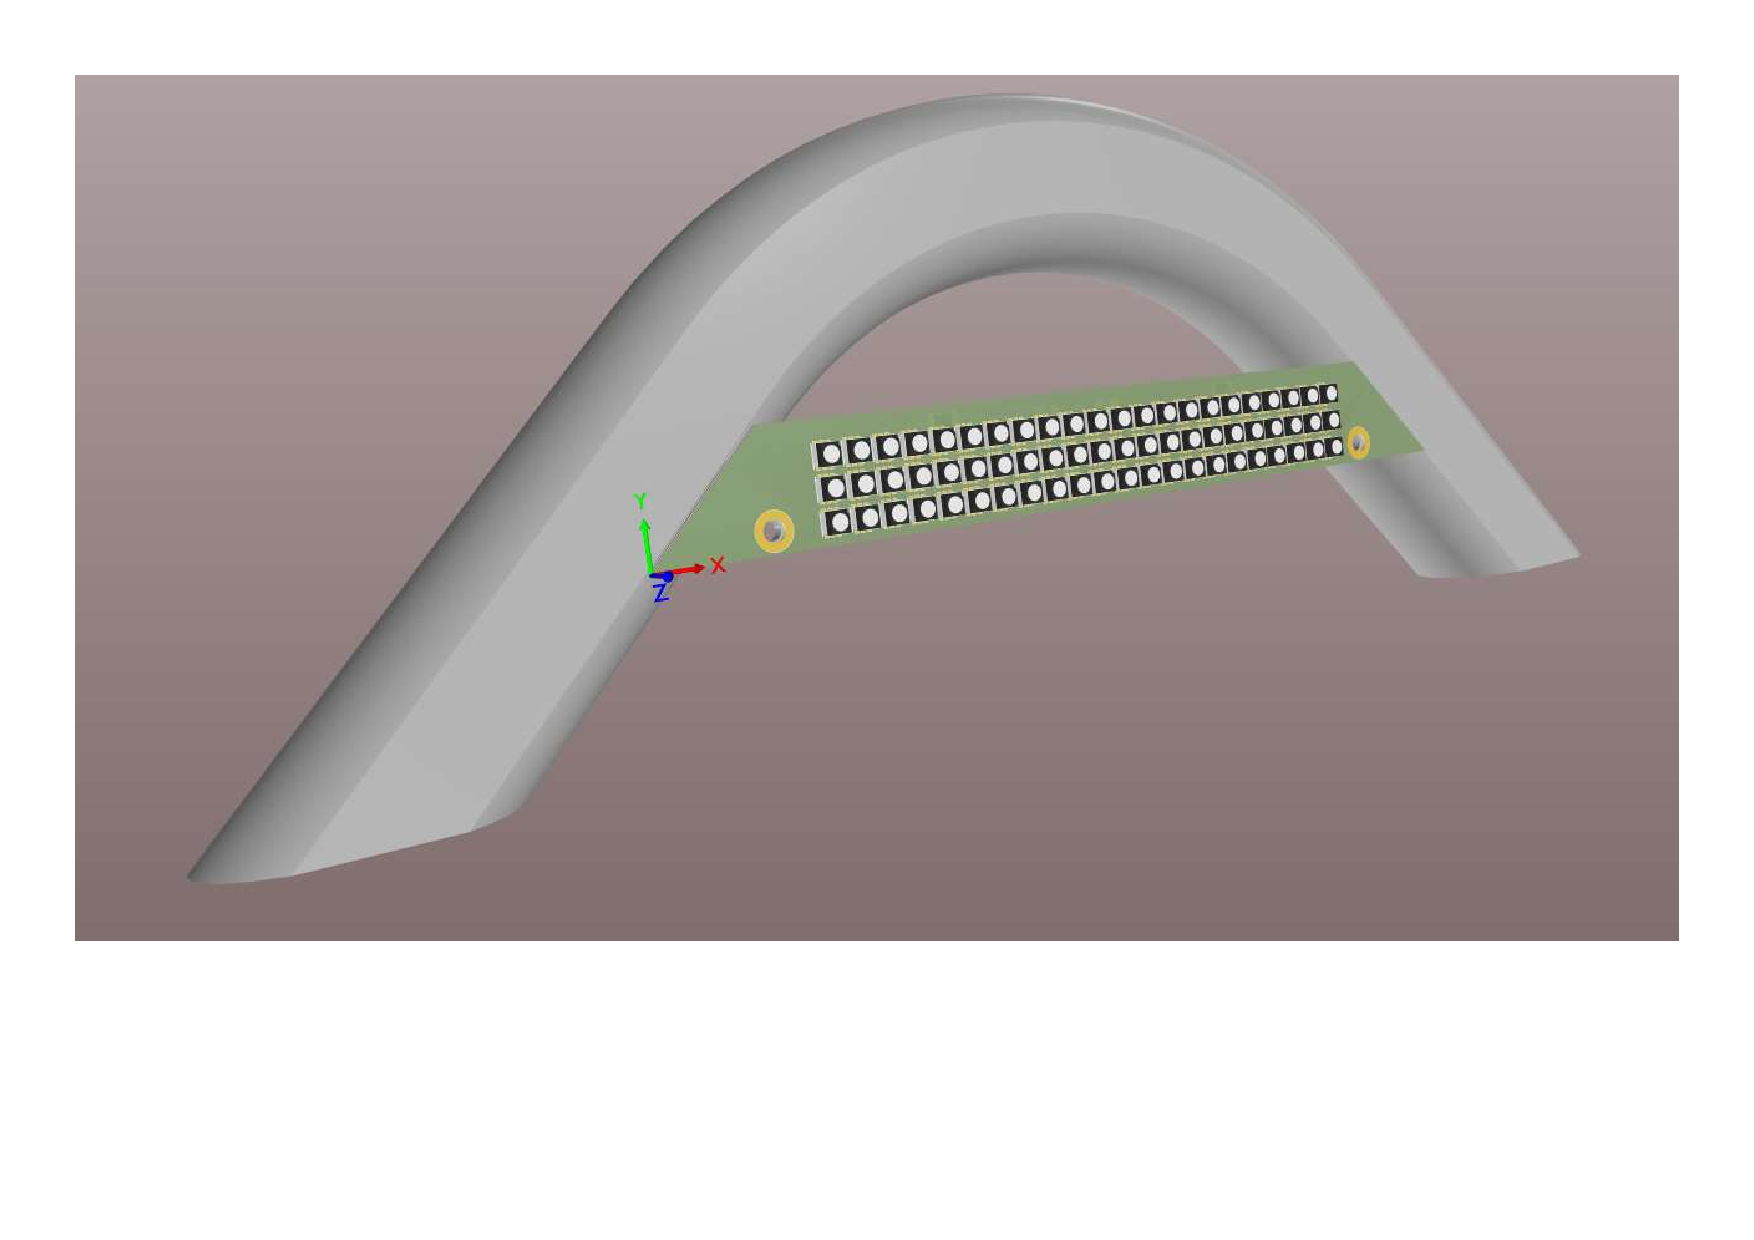
\includegraphics[width=\textwidth,trim={3cm 11cm 2cm 1cm},clip]{./img/tsal-position.pdf}
	\caption{TSAL position.}
	\label{fig:TSAL-position}
\end{figure}